\documentclass[12pt, twoside]{article}
\usepackage[letterpaper, margin=1in, headsep=0.5in]{geometry}
\usepackage[english]{babel}
\usepackage[utf8]{inputenc}
\usepackage{amsmath}
\usepackage{amsfonts}
\usepackage{amssymb}
\usepackage{tikz}
%\usetikzlibrary{quotes, angles}

\usepackage{graphicx}
\usepackage{enumitem}
\usepackage{multicol}

\usepackage{fancyhdr}
\pagestyle{fancy}
\fancyhf{}
\renewcommand{\headrulewidth}{0pt} % disable the underline of the header

\fancyhead[RE]{\thepage}
\fancyhead[RO]{\thepage \\ Name: \hspace{3cm}}
\fancyhead[L]{BECA / Dr. Huson / 10th Grade Geometry\\* 10 June 2019}

\begin{document}
\subsubsection*{13-7 Do Now: Transformations, symmetry}
Use only a compass and straightedge for these constructions. [Leave all construction marks.]
 \begin{enumerate}

  \item In the circle below, $\overline{AB}$ is a chord. Using a compass and straightedge, construct a perpendicular bisector of $\overline{AB}$, and hence, a diameter of the circle. \vspace{1cm}
   \begin{center}
   \begin{tikzpicture}[scale=.635]
     %\draw [help lines] (-4,-4) grid (4,4);
     \draw [thick, -] (80:5) node[above right]{$A$} -- (-20:5) node[right]{$B$};
     %\draw [thick, ->] (0,-2.2)--(0,10.4) node [left] {$y$};
     \draw (0,0) circle [radius=5]; %node[below]{$C$};
     %\draw [fill] (0,0) circle [radius=0.05];
   \end{tikzpicture}
 \end{center} \vspace{1cm}

   \item Given the points $A$, $B$, and $C$ as shown, construct the parallelogram $ABCD$.
   \vspace{1cm}
    \begin{center}
    \begin{tikzpicture}[scale=1.2]
      \draw [fill] (1,-2) circle [radius=0.05] node[below left]{$A$};
      \draw [fill] (4,2) circle [radius=0.05] node[above]{$B$};
      \draw [fill] (8,1) circle [radius=0.05] node[right]{$C$};
    \end{tikzpicture}
    \end{center}

\newpage
\item Construct the line of reflection used when $\triangle ABC$ is reflected onto $\triangle A'B'C'$.\vspace{0.5cm}
    \begin{center}
    \begin{tikzpicture}[scale=.8, rotate=110]
      %\draw [dashed, <->] (-1,-1)--(7,7) node[below right]{$l$};
      \draw [thick]
      (5,-1) node[below right] {$A$}--
      (7,2) node[above] {$B$}--
      (2,0) node[below right] {$C$}--cycle;
      \draw [thick]
      (-1,5) node[below] {$A'$}--
      (2,7) node[above left] {$B'$}--
      (0,2) node[below right] {$C'$}--cycle;
    \end{tikzpicture}
  \end{center} \vspace{1cm}

  \item The vertices of $\triangle JKL$ have the coordinates $J(-4,4)$, $K(2,-2)$, and $L(2,4)$, as shown. \\[0.25cm]
    Apply a dilation to $\triangle JKL \rightarrow \triangle J'K'L'$, centered on $(2,1)$ with a scale factor $k=\frac{4}{3}$. Draw the image $\triangle J'K'L'$ on the set of axes below, labeling the vertices.
    \begin{center}
      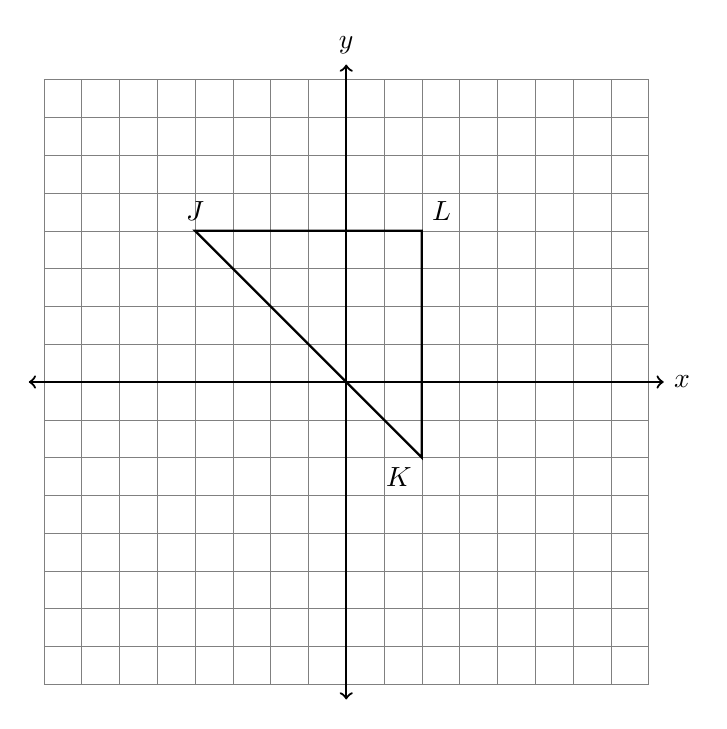
\begin{tikzpicture}[scale=.48]
        \draw [help lines] (-8,-8) grid (8,8);
        \draw [thick, <->] (-8.4,0) -- (8.4,0) node [right] {$x$};
        \draw [thick, <->] (0,-8.4)--(0,8.4) node [above] {$y$};
        \draw [thick]
        (-4,4) node[above] {$J$}--
        (2,-2) node[below left] {$K$}--
        (2,4) node[above right] {$L$}--
        cycle;
      \end{tikzpicture}
    \end{center}

\newpage

  \item What transformation(s) map $\triangle ABC$ onto $\triangle DEF$, shown below? Fully specify the transformations.
    \begin{center}
      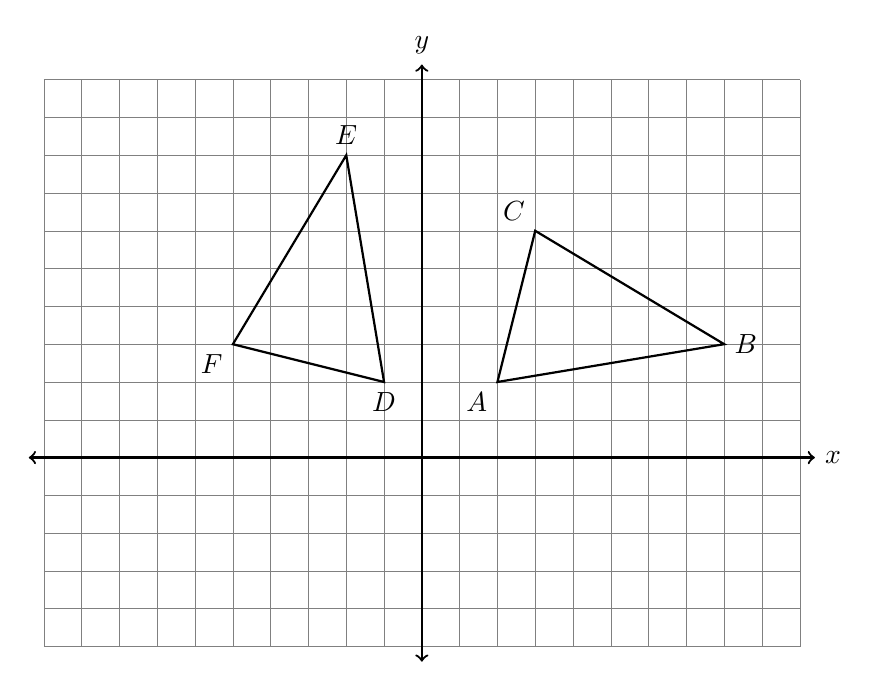
\begin{tikzpicture}[scale=.48]
        \draw [help lines] (-10,-5) grid (10,10);
        \draw [thick, <->] (-10.4,0) -- (10.4,0) node [right] {$x$};
        \draw [thick, <->] (0,-5.4)--(0,10.4) node [above] {$y$};
        \draw [thick]
          (2,2) node[below left] {$A$}--
          (8,3) node[right] {$B$}--
          (3,6) node[above left] {$C$}--cycle;
        \draw [thick]
          (-1,2) node[below] {$D$}--
          (-2,8) node[above] {$E$}--
          (-5,3) node[below left] {$F$}--cycle;
      \end{tikzpicture}
    \end{center}
      \vspace{2cm}

  \item A translation maps $A(5,-1) \rightarrow A'(5,7)$. What is the image of $B(-1,7)$ under the same translation?  \vspace{2cm}

  \begin{multicols}{2} [\item Circle YES or NO to indicate whether the given transformation maps the pentagon onto itself.] %$ABCDEF$
  \vspace{0.5cm}
   \begin{enumerate}
     \item Yes \quad No \quad A rotation of $60^\circ$ clockwise around the pentagon's center.
      \item Yes \quad No \quad A reflection over $\overleftrightarrow{AD}$
      \item Yes \quad No \quad A reflection over a line through the midpoint of  $\overline{AE}$ and $C$.
      \item Yes \quad No \quad A rotation of $144^\circ$ counterclockwise around the pentagon's center.
      \end{enumerate}
    \begin{center}
        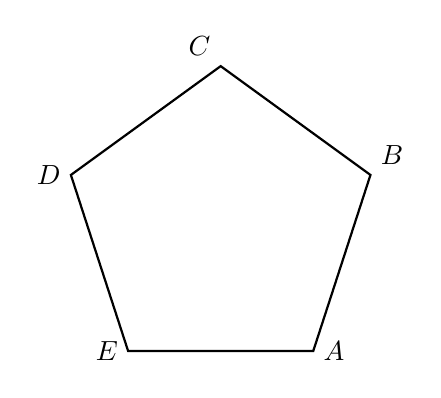
\begin{tikzpicture}%[scale=.48]
          \draw [thick]
          (-54:2)node[right] {$A$}--
          (18:2)node[above right] {$B$}--
          (90:2)node[above left] {$C$} --
          (162:2)node[left] {$D$}--
          (234:2)node[left] {$E$}--cycle;
          %(300:2)node[right] {$F$}--cycle;
        \end{tikzpicture}
      \end{center}
    \end{multicols} \vspace{0.5cm}

\newpage

  \item What is the equation of a line resulting when the line $y=\frac{1}{3}x-3$ is dilated by a factor of 3 centered at the origin?
  \vspace{2cm}

  \item Directed line segment $DE$ has endpoints $D(-4,-2)$ and $E(1,8)$. Point $F$ divides $\overline{DE}$ such that $DF{:}FE$ is $2{:}3$. What are the coordinates of $F$? \vspace{4cm}

  \item The figure shows a rectangle (not a square).
   \begin{center}
     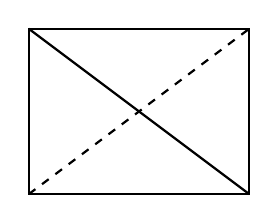
\begin{tikzpicture}[scale=0.7]
       \coordinate (A) at (0, 0); %[label=above left:$P$]
       \coordinate (B) at (4, 0);
       \coordinate (C) at (4, 3);
       \coordinate (D) at (0, 3);
       \draw [thick] (A)--(B)--(C)--(D)--cycle;
       \draw [thick, dashed] (A)--(C);
       \draw [thick] (B)--(D);
       %\draw [thick, xshift=2cm, yshift=2.5cm] (85:3);
     \end{tikzpicture}
   \end{center}
   Which transformations carry the rectangle onto itself? Mark each True or False.
     \begin{enumerate}
       \item A reflection one of the longer sides \hfill True \quad False
       \item A reflection over the dashed diagonal \hfill True \quad False
       \item A clockwise rotation of $90^\circ$ about the intersection of the diagonals \hfill True \quad False
       \item A clockwise rotation of $180^\circ$ about the intersection of the diagonals \hfill True \quad False
     \end{enumerate}
     \vspace{1cm}

   \item What is the smallest non-zero angle of rotation about its center that would map the nonagon onto itself? \vspace{0.25cm} %$ABCDE$
   \begin{center}
      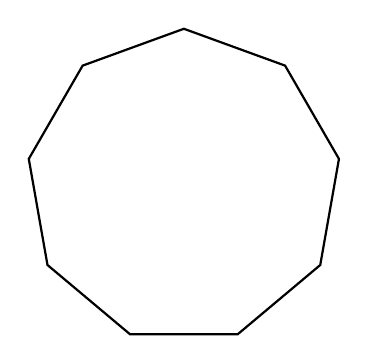
\begin{tikzpicture}%[scale=.48]
        \draw [thick]
        (10:2)--% node[right] {$A$}--
        (50:2)--% node[above right] {$B$}--
        (90:2)--% node[above left] {$C$} --
        (130:2)--% node[left] {$D$}--
        (170:2)--
        (210:2)--
        (250:2)--
        (290:2)--
        (330:2)--cycle;% node[right] {$E$}--cycle;
      \end{tikzpicture}
    \end{center}

\end{enumerate}
\newpage
\setcounter{page}{1}
\subsubsection*{13.7 Exit Note Quiz: Transformations, symmetry}
Use only a compass and straightedge for these classical constructions, showing all construction marks.
 \begin{enumerate}

  \item In the circle below, $\overline{AB}$ is a chord. Using a compass and straightedge, construct a perpendicular bisector of $\overline{AB}$, and hence, a diameter of the circle. \vspace{2cm}
    \begin{center}
    \begin{tikzpicture}[scale=.635]
      %\draw [help lines] (-4,-4) grid (4,4);
      \draw [thick, -] (-5,0) node[left]{$A$} -- (0,5) node[above]{$B$};
      %\draw [thick, ->] (0,-2.2)--(0,10.4) node [left] {$y$};
      \draw (0,0) circle [radius=5]; %node[below]{$C$};
      %\draw [fill] (0,0) circle [radius=0.05];
    \end{tikzpicture}
    \end{center} \vspace{1cm}

  \item Given the points $A$, $B$, and $C$ as shown, construct the parallelogram $ABCD$.
    \vspace{3cm}
   \begin{center}
   \begin{tikzpicture}[scale=1.2]
     \draw [fill] (0,0) circle [radius=0.05] node[below left]{$A$};
     \draw [fill] (6,-2) circle [radius=0.05] node[below]{$B$};
     \draw [fill] (6,1) circle [radius=0.05] node[right]{$C$};
   \end{tikzpicture}
   \end{center}

\newpage
  \item Construct the line of reflection used when $\triangle ABC$ is reflected onto $\triangle A'B'C'$.\vspace{0.5cm}
     \begin{center}
     \begin{tikzpicture}[scale=.8]
       %\draw [dashed, <->] (-1,-1)--(7,7) node[below right]{$l$};
       \draw [thick]
       (5,-1) node[below right] {$A$}--
       (7,2) node[right] {$B$}--
       (1,0) node[below left] {$C$}--cycle;
       \draw [thick]
       (-1,5) node[left] {$A'$}--
       (2,7) node[above left] {$B'$}--
       (0,1) node[below left] {$C'$}--cycle;
     \end{tikzpicture}
   \end{center} \vspace{1cm}

 \item The vertices of $\triangle JKL$ have the coordinates $J(-4,1)$, $K(2,-2)$, and $L(2,4)$, as shown. \\[0.25cm]
   Apply a dilation to $\triangle JKL \rightarrow \triangle J'K'L'$, centered on $(-2,2)$ with a scale factor $k=1.5$. Draw the image $\triangle J'K'L'$ on the set of axes below, labeling the vertices.
   \begin{center}
     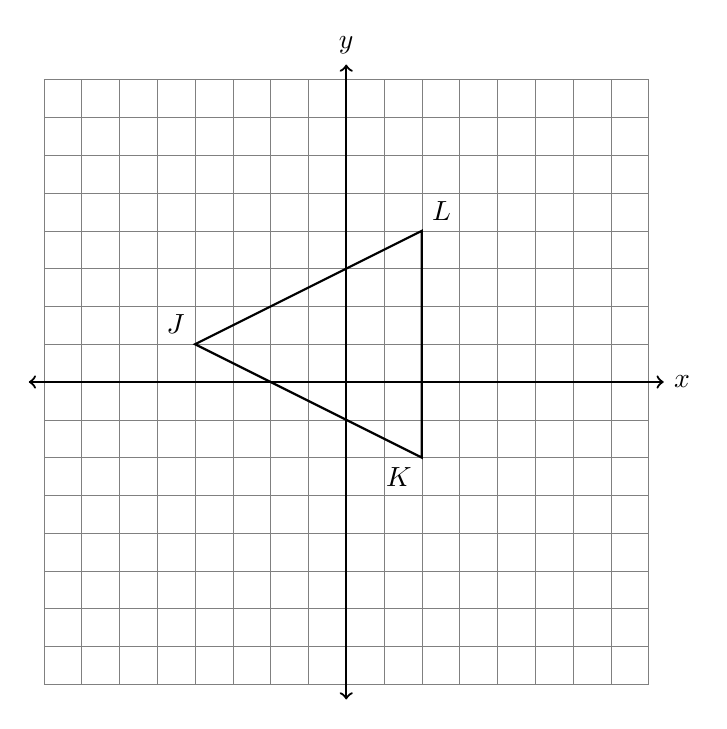
\begin{tikzpicture}[scale=.48]
       \draw [help lines] (-8,-8) grid (8,8);
       \draw [thick, <->] (-8.4,0) -- (8.4,0) node [right] {$x$};
       \draw [thick, <->] (0,-8.4)--(0,8.4) node [above] {$y$};
       \draw [thick]
       (-4,1) node[above left] {$J$}--
       (2,-2) node[below left] {$K$}--
       (2,4) node[above right] {$L$}--
       cycle;
     \end{tikzpicture}
   \end{center}

\newpage

 \item What transformation(s) map $\triangle ABC$ onto $\triangle DEF$, shown below? Fully specify the transformations.
   \begin{center}
     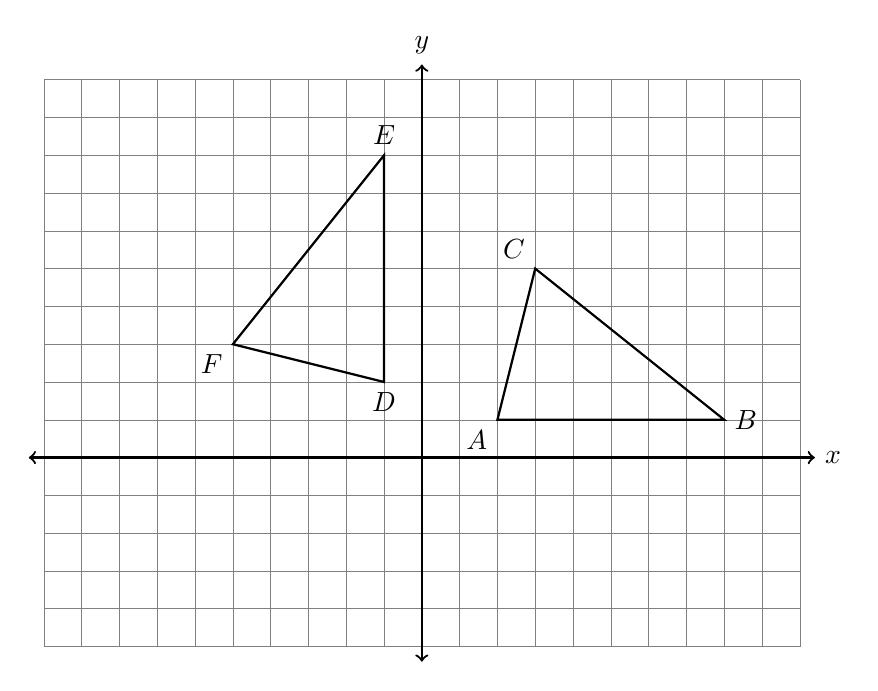
\begin{tikzpicture}[scale=.48]
       \draw [help lines] (-10,-5) grid (10,10);
       \draw [thick, <->] (-10.4,0) -- (10.4,0) node [right] {$x$};
       \draw [thick, <->] (0,-5.4)--(0,10.4) node [above] {$y$};
       \draw [thick]
         (2,1) node[below left] {$A$}--
         (8,1) node[right] {$B$}--
         (3,5) node[above left] {$C$}--cycle;
       \draw [thick]
         (-1,2) node[below] {$D$}--
         (-1,8) node[above] {$E$}--
         (-5,3) node[below left] {$F$}--cycle;
     \end{tikzpicture}
   \end{center}
     \vspace{2cm}

 \item A translation maps $A(6,-2) \rightarrow A'(-2,6)$. What is the image of $B(-2,6)$ under the same translation?  \vspace{2cm}

 \begin{multicols}{2} [\item Circle YES or NO to indicate whether the given transformation maps the hexagon onto itself.] %$ABCDEF$
 \vspace{0.5cm}
  \begin{enumerate}
    \item Yes \quad No \quad A rotation of $120^\circ$ counterclockwise around point $D$.
     \item Yes \quad No \quad A reflection over $\overleftrightarrow{AE}$
     \item Yes \quad No \quad A reflection over a line through the midpoints of  $\overline{BC}$ and $\overline{EF}$.
     \item Yes \quad No \quad A rotation of $60^\circ$ clockwise around the hexagon's center.
     \end{enumerate}
   \begin{center}
       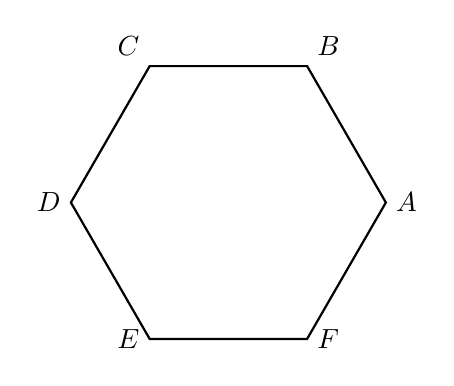
\begin{tikzpicture}%[scale=.48]
         \draw [thick]
         (0:2)node[right] {$A$}--
         (60:2)node[above right] {$B$}--
         (120:2)node[above left] {$C$} --
         (180:2)node[left] {$D$}--
         (240:2)node[left] {$E$}--
         (300:2)node[right] {$F$}--cycle;
       \end{tikzpicture}
     \end{center}
   \end{multicols} \vspace{0.5cm}

\newpage

 \item What is the equation of a line resulting when the line $y=-2x+4$ is dilated by a factor of $\frac{3}{2}$ centered at the origin?
 \vspace{2cm}

 \item Directed line segment $DE$ has endpoints $D(-2,-1)$ and $E(4,8)$. Point $F$ divides $\overline{DE}$ such that $DF{:}FE$ is $1{:}2$. What are the coordinates of $F$? \vspace{4cm}

 \item The figure shows a rectangle (not a square).
  \begin{center}
    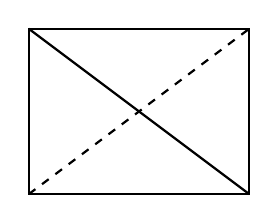
\begin{tikzpicture}[scale=0.7]
      \coordinate (A) at (0, 0); %[label=above left:$P$]
      \coordinate (B) at (4, 0);
      \coordinate (C) at (4, 3);
      \coordinate (D) at (0, 3);
      \draw [thick] (A)--(B)--(C)--(D)--cycle;
      \draw [thick, dashed] (A)--(C);
      \draw [thick] (B)--(D);
      %\draw [thick, xshift=2cm, yshift=2.5cm] (85:3);
    \end{tikzpicture}
  \end{center}
  Which transformations carry the rectangle onto itself? Mark each True or False.
    \begin{enumerate}
      \item A reflection over the solid diagonal \hfill True \quad False
      \item A reflection over the dashed diagonal \hfill True \quad False
      \item A clockwise rotation of $360^\circ$ about the intersection of the diagonals \hfill True \quad False
      \item A clockwise rotation of $180^\circ$ about the intersection of the diagonals \hfill True \quad False
    \end{enumerate}
    \vspace{1cm}

  \item What is the smallest non-zero angle of rotation about its center that would map the pentagon onto itself? \vspace{0.25cm} %$ABCDE$
  \begin{center}
     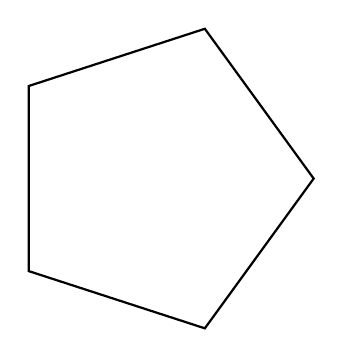
\begin{tikzpicture}%[scale=.48]
       \draw [thick]
       (0:2)--% node[right] {$A$}--
       (72:2)--% node[above right] {$B$}--
       (144:2)--% node[above left] {$C$} --
       (216:2)--% node[left] {$D$}--
       (288:2)--cycle;% node[right] {$E$}--cycle;
     \end{tikzpicture}
   \end{center}

\end{enumerate}
\end{document}
